\documentclass[english]{scrartcl}
\usepackage[T1]{fontenc}
\usepackage{listings}
\usepackage{hyperref}
\usepackage{graphicx}
\usepackage{color}
\usepackage{soul}
\usepackage{seqsplit}
\usepackage{multirow}
\usepackage{enumitem}
\usepackage{graphicx}
\usepackage{float}
\usepackage{amsmath}




\begin{document}
\section*{Task 8}

The experiment was hold with folding ruler with two joints. Firstly, markers on the parts of the ruler were aligned. At first both joints were recognised as rigid. After collecting 50 poses recognition has started.
\\
Selecting kinematic graph (fast)
\\
spanning tree: 1-DOF (ro:0,1),(ri:1,2)
\\
starting from current graph: 1-DOF (ro:0,1),(ri:1,2)
\\
finding neighbors, total graphs = 6
\\
 \t starting   -73.5558  1-DOF (ro:0,1),(ri:1,2) pos=0.00275962 orient=0.061114
 \\
 \t evaluating -63.9391 (2-DOF (ro:0,1/3),(ro:0,2/3),(ri:1,2/3) pos=0.00226167 orient=0.0858353
\\
-73.5558  1-DOF (ro:0,1),(ri:1,2)
\\
final:  -73.5558  1-DOF (ro:0,1),(ri:1,2) pos=0.00275962 orient=0.061114 stamps=3
\\
 evals: 1
\\
So the graph was build and then evaluated. After that BICs are counted and the best graph is selected as resulting. At the same time this graph is visualised in the window of the program as in Figure \ref{fig:graph}.

\begin{figure}[h]
\centering
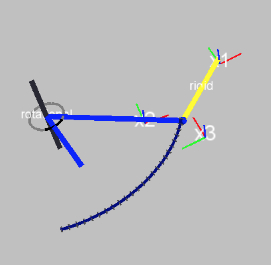
\includegraphics{./graph}
\caption{Visualised graph for kinematic model}
\label{fig:graph}
\end{figure}

Finally the ruler was recognised as one rotational joint and one rigid. The result was not changed after several experiments also.
\end{document}





